\documentclass[%
reprint,
superscriptaddress,
%groupedaddress,
%unsortedaddress,
%runinaddress,
%frontmatterverbose, 
%preprint,
%preprintnumbers,
%nofootinbib,
%nobibnotes,
%linenumbers,
%bibnotes,
amsmath,amssymb,
aps,
pra,
%prb,
%rmp,
%prstab,
%prstper,
%floatfix,
]{revtex4-2}

\usepackage{graphicx}% Include figure files
\usepackage{dcolumn}% Align table columns on decimal point
\usepackage{bm}% bold math
\usepackage{xcolor}
\usepackage{braket}
\usepackage{float}
\usepackage{lipsum}
\usepackage{caption}
\usepackage{subcaption}
\usepackage{mathtools}
\usepackage{float} % Para o [H]
%\usepackage{hyperref}% add hypertext capabilities
%\usepackage[mathlines]{lineno}% Enable numbering of text and display math
%\linenumbers\relax % Commence numbering lines

%\usepackage[showframe,%Uncomment any one of the following lines to test 
%%scale=0.7, marginratio={1:1, 2:3}, ignoreall,% default settings
%%text={7in,10in},centering,
%%margin=1.5in,
%%total={6.5in,8.75in}, top=1.2in, left=0.9in, includefoot,
%%height=10in,a5paper,hmargin={3cm,0.8in},
%]{geometry}

\begin{document}
\preprint{APS/123-QED}

\title{Dissipative charging of bosonic quantum batteries via nonequilibrium gain and loss}% Force line breaks with \\
%\thanks{A footnote to the article title}%

\author{A. E. B. Costa}
\affiliation{Instituto Federal de Alagoas, Maceió, Brasil}
\author{I. Beder}
\affiliation{Instituto de F\'isica, Universidade Federal de Alagoas, Macei\'o, Brasil}
\affiliation{Instituto de F\'isica, Universidade Federal de Alagoas, Macei\'o, Brasil}

\author{P. A. Brand\~ao}
 \email{paulo.brandao@fis.ufal.br}
 \affiliation{Instituto de F\'isica, Universidade Federal de Alagoas, Macei\'o, Brasil}
 

\date{\today}% It is always \today, today,
             %  but any date may be explicitly specified

\begin{abstract}
We investigate the dissipative charging dynamics of a bosonic quantum battery interacting with two Markovian reservoirs: one inducing energy gain and the other inducing loss, both described by identical rates $\gamma$, thereby realizing a $PT$-symmetric dissipative configuration. When the battery is initially empty, we observe a monotonic increase of the internal energy over time $t$ while the ergotropy remains strictly zero during the charging protocol. For initially populated Fock states with $k$ excitations, the ergotropy decreases and vanishes for $\gamma t \geq k$, indicating a complete loss of extractable work despite continuous energy input. We further examine the role of initial quantum coherences in the battery state and find that \textcolor{red}{XXXX}. Our results highlight fundamental limitations on work extraction from dissipatively charged quantum systems, even under symmetric and energy-preserving environmental configurations.
\end{abstract}

%\keywords{Suggested keywords}%Use showkeys class option if keyword
                              %display desired
\maketitle

%\tableofcontents

\section{Introduction}

A quantum battery (QB) is an energy-storage device that, distinct from its classical counterpart, takes advantage of quantum phenomena, such as entanglement, to boost its performance \cite{alicki2013entanglement, campaioli2024colloquium}. One of the main figures of merit characterizing the state of a QB is the ergotropy $\mathcal{E}$. It quantifies the amount of work (useful energy) that can be extracted from the QB by a unitary cyclic process \cite{allahverdyan2004maximal}. The role of coherence and entanglement in work extraction processes has been the central topic of intense research in the past few years [] and a host of physical systems that could act as a QB have been proposed, including spin-based QB [], (...) 

A charging protocol is usually considered in which the QB, initially empty, interacts with another (quantum or classical) system, called the charger, that holds some energy before the interaction takes place. This energy is transferred to the QB in the hope that it becomes extractable, that is, with nonzero ergotropy. 


\section{Theory}

\subsection{Collision Model}

Consider a QB composed of a single-mode harmonic oscillator having frequency $\omega$ and Hamiltonian $H_S = \omega b^{\dagger}b$, where $b$ is the annihilation operator and $\hbar = 1$ hereafter. The QB interacts simultaneously with two atomic baths composed of excited and ground state two-level systems, described by the Hamiltonians $H_G$ and $H_L$, respectively, as depicted in Fig. \ref{fig1}. Each bath is formed by discrete ancillas that interact with the QB during a collision time $\tau$. The initial state of the total system is given by
\begin{equation}
    \rho_{SB}(0) = \rho_S(0)\, \otimes \, \rho_G(0) \, \otimes \, \rho_L(0),
\end{equation}
 where $B$ indicates the baths $G$ and $L$ and $\rho_j(0)$ ($j = S$, $G$, $L$) is the initial density operator of system $j$. Each ancilla of the $G$ bath starts in the excited state $\ket{e_G}$, so that $\rho_G(0) = \bigotimes_{n}\ket{e_G^n}\bra{e_G^n}$ and each ancilla of the $L$ bath starts in the ground state $\ket{g_L}$, so that $\rho_L(0) = \bigotimes_{n}\ket{g_L^n}\bra{g_L^n}$.


\begin{figure}[H]
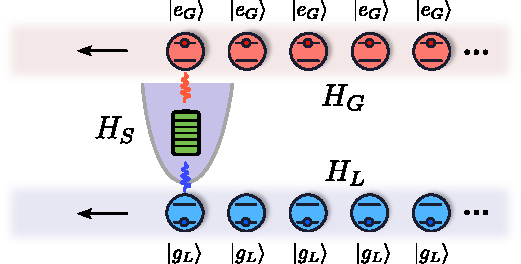
\includegraphics[width=0.9\linewidth]{fig1.pdf}
\caption{A bosonic quantum battery, with Hamiltonian $H_S = \omega b^{\dagger}b$, (a single-mode cavity field) interacts with two atomic nonequilibrium baths. The gain bath consists of a sequence of excited atoms, described by the Hamiltonian $H_G$, which may increase photon excitations. The loss bath, characterized by the Hamiltonian $H_L$, is formed by ground state atoms that may absorb photonic excitations. The ancillas composing both baths do not interact between each other and are coupled to the quantum battery during a collision time $\tau$.}
\label{fig1} 
\end{figure}

The interaction energy between each individual ancilla and the QB is given by 
\begin{equation}
    H_{Sj}^n = g_j(b^{\dagger} \sigma_{j,n}^{-} + b\sigma_{j,n}^{+}) \quad (j = G,L),
\end{equation}
where $g_j$ is the coupling parameter between the QB and the reservoir $j=G,L$ and $\sigma^{\pm}$ are the Pauli raising and lowering operators for the qubits. The collision model assumes a discrete time $t_n = n\tau$ for the interaction between the QB and the ancillas. That is, the pair of ancillas $n$, one from each bath, interacts with the QB in the time interval $[(n-1)\tau, n\tau]$. In this interval, the total system evolves as $\rho_{SB}(n) = U(n) \rho_{SB}[(n-1)] U(n)^{\dagger}$, where $U(n)$ is the time-evolution operator
\begin{equation}
    U(n) = e^{-i\tau(H_S + H_{G,n} + H_{L,n} + H^n_{SG} + H^n_{SL})},
\end{equation} 
where $H_{j,n} = (\omega/2)\sigma^{z}_{j,n}$ $(j=G,L)$ is the atomic energy of the $n$th qubit in bath $j$. Notice that we assume a ressonant interaction between each ancilla and the QB. The density operator $\rho(n)$ for the QB after $n$ interactions can be obtained by taking the partial trace $\rho(n) = \text{Tr}_{B}[\rho_{SB}(n)]$.

Under these assumptions (one collision between each ancilla and the QB, forbidden ancilla-ancilla interaction and uncorrelated initially prepared ancillas), it is known that this collision model generates a Markovian dynamics where each collision is fully characterized by a CPTP map ~\cite{ciccarello2022quantum}. 

%\begin{figure}[H]
%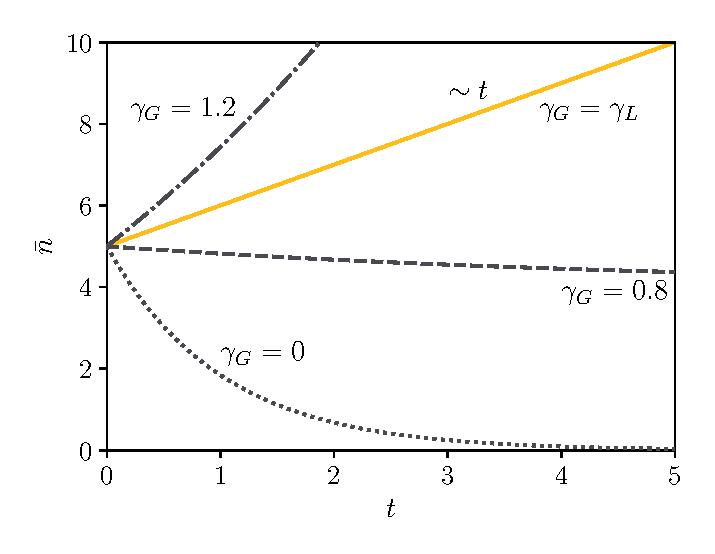
\includegraphics[width=\linewidth]{fig2.eps}
%\caption{Plots of $\bar{n}(t)$ as a function of time $t$ for (dotted line) $\gamma_G = 0$, (dashed line) $\gamma_G = 0.8$, (solid line) $\gamma_G = \gamma_L$ and (dash-dot line) $\gamma_G = 1.2$. The value of $\gamma_L = 1$ is fixed. The asymptotic value for the case $\gamma_G = 0.8$ is given by $\gamma_G/(\gamma_L - \gamma_G) = 4$. The averaged number of initial photons is $\bar{n}(0) = 5$. A charging (discharging) dynamics occurs for $\gamma_G \geq \gamma_L$ ($\gamma_G < \gamma_L$).}
%\label{fig2}
%\end{figure} 


\subsection{Ergotropy}

The ergotropy $\mathcal{E}$ is an important figure of merit that characterizes the maximum amount of work that can be extracted from a given quantum state $\hat{\rho}$ of the QB under a cyclic and unitary transformation \cite{allahverdyan2004maximal}. It is defined by $$\mathcal{E} = \text{Tr}(\rho H) - \underset{U}{\min} \text{Tr}(U \rho U^{\dagger} H),$$ where the minimization is over all possible unitary transformations $U$. A more tractable formula for $\mathcal{E}$ can be written in terms of the passive state $\sigma$ of $\rho$, defined by
\begin{align}
    \sigma = \sum_{n = 0}\lambda_n\ket{n}\bra{n}
\end{align}
where $\lambda_n$ are the eigenvalues of $\hat{\rho}$ rearranged in decreasing order, $\lambda_n > \lambda_{n+1}$ and $\{ \ket{n} \}$ is the Hamiltonian eigenbasis. The ergotropy can thus be evaluated as
\begin{align}\label{ergotropy}
    \mathcal{E} = \text{Tr}(\rho H) - \text{Tr}( \sigma H).
\end{align}

In the next section, we explore the role of the ergotropy $\mathcal{E}$ and the energy $E$ in the charging protocol of the QB interacting with the gain and loss atomic baths. 

\section{Results and discussion}

\subsection{One-cell quantum battery }
Let us start by assuming that the QB is initially in the vacuum state $\hat{\rho}(0) = \ket{0}\bra{0}$. As discussed in the previous section, the energy of the battery will then increase during the charging protocol and we are interested in the fraction of this energy that can be extracted as work, given by Eq. \eqref{ergotropy}. The inset of Fig. \ref{fig3} shows the energy $E$ (gray line) and the ergotropy $\mathcal{E}$ (red line) as a function of $\gamma t$.  It is clear from these plots that the energy increases but the ergotropy remains zero, so that no work can be extracted after the charging protocol is completed.

\begin{figure}[H]
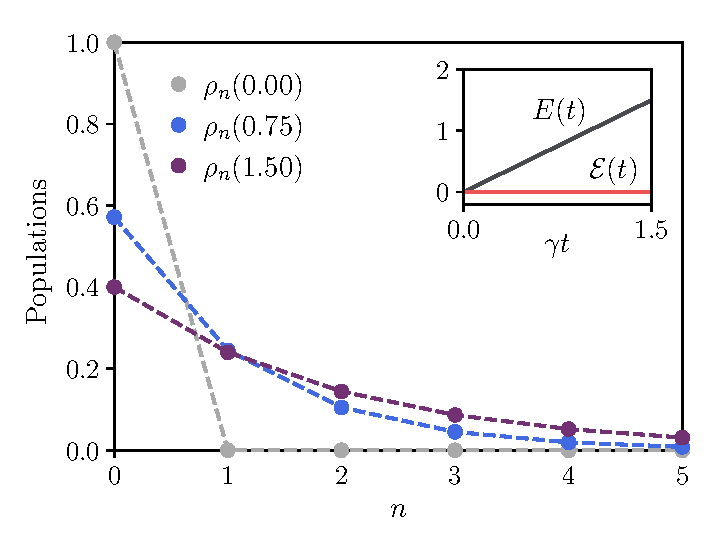
\includegraphics[width=\linewidth]{fig3.eps}
\caption{Charging of a bosonic QB that is initially in the vacuum state $\hat{\rho}(0) = \ket{0}\bra{0}$. The plot displays the populations $\rho_{n}(t) = \bra{n}\hat{\rho}(t)\ket{n}$ as a function of the occupation number $n$ for $\gamma t = 0$ (gray dots), $\gamma t = 7.5$ (blue dots) and $\gamma t = 15$ (purple dots). The inset shows the energy $E$ and ergotropy $\mathcal{E}$ in units of $\omega$ as a function of $\gamma t$. }
\label{fig3}
\end{figure}

To explain this behavior, we focus on the evolution of the populations $\rho_n(t) = \bra{n}\hat{\rho}(t)\ket{n}$. Since the initial state of the QB is diagonal in the energy basis of the Hamiltonian, the eigenvalues of $\hat{\rho}$ are identified with the populations $\rho_n$. Figure \ref{fig3} shows the populations $\rho_n$ as a function of the mode number $n$ for fixed charging times $\gamma t = 0$ (gray dots), $\gamma t = 0.75$ (blue dots) and $\gamma t = 1.5$ (purple dots). Initially, only the mode $n = 0$ is excited, as expected. As $t$ increases, there is a redistribution of populations throughout excited states $(n>0)$, but, as is evident from the plots, the distribution follows an exponentially decreasing function of $n$, which suggests that the state of the quantum battery evolves to a thermal-like state distribution. Thus, a non-Hermitian-induced thermalization precludes the extraction of work. The same behavior was observed for the case $\gamma_G > \gamma_L$, except that the modes $\rho_n$ are populated faster than the $PT$-symmetric case.

The exact thermal distribution can be obtained directly from Eq. \eqref{mk} by fixing $k = 0$ and expanding $M_k(\mu,t)$ in a power series of $(1-\mu)^n$. The populations are given by
\begin{equation}
    \rho^{(k=0)}_n (t) = \frac{(\gamma t)^{n}}{(1 + \gamma t)^{n+1}},
\end{equation}
which describes a thermal distribution having mean photon number $\bar{n} = \gamma t$, which can be directly obtained from Eq. \eqref{navt} by taking $\gamma_L = \gamma_G = \gamma$ and $\bar{n}(0) = 0$. Thus, the passive state is obviously $\hat{\sigma} = \rho_n^{(k=0)}$ and the ergotropy vanishes at all times if the QB is initially in the vacuum state.


\begin{figure}[H]
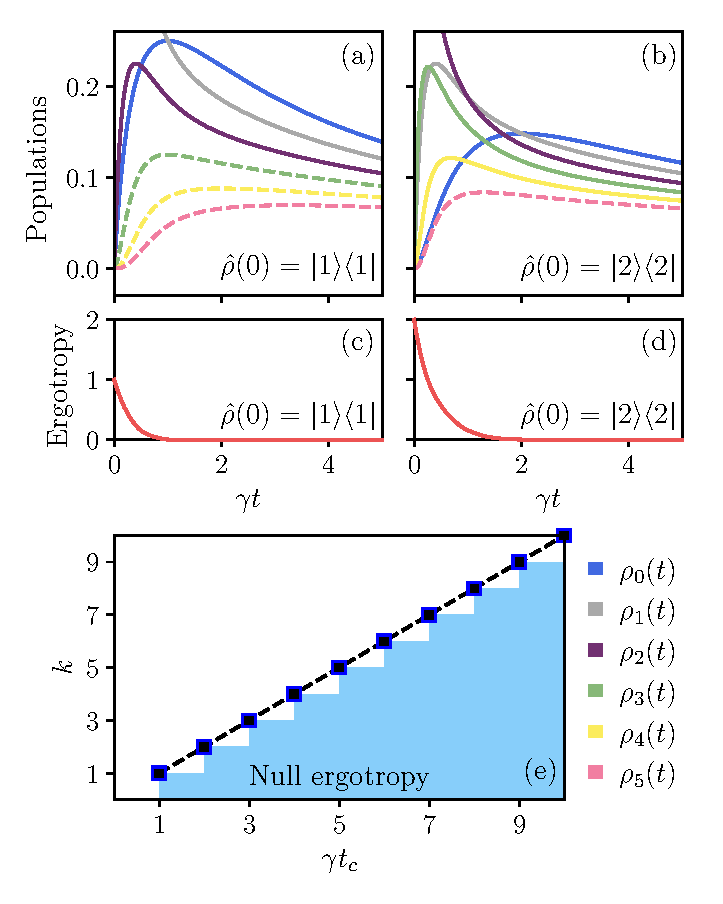
\includegraphics[width=\linewidth]{fig4.eps}
\caption{caption}
\label{fig4}
\end{figure}

We see that the energy deposited in the QB by the PT-symmetric reservoir is useless because it creates thermal-like states with zero ergotropy. What happens then if the QB has initially some energy and ergotropy? To explore this situation, let us consider the simplest case where the QB initially holds a single photon, that is, $\hat{\rho}(0) = \ket{1}\bra{1}$. Equation \eqref{mk} can then be used with $k = 1$ to extract the populations, 
\begin{equation}
    \rho_n^{(k=1)}(t) = \Bigg( \gamma t + \frac{n}{\gamma t} \Bigg) \frac{(\gamma t)^n}{(1+\gamma t)^{n+2}}.
\end{equation}
Figure \ref{fig4} plots the ergotropy $\mathcal{E}$ as a function of $\gamma t$. The plot clearly suggests an exponential \textit{discharging} dynamics (in the sense that the ergotropy is being drained during the time period), even though the energy is increasing. Note, however, that this is not technically an exponential behavior for all times. The ergotropy exactly vanishes at $\gamma t_c = 1$. This can be seen by inspecting the plots of the populations and searching for the time $t_c$ where the curves for $\rho_0$ and $\rho_1$ cross each other. The time $t_c$ also happens to be the time where the ergotropy vanishes. 

The exact time $t_c$ for which $\mathcal{E}(t_c) = 0$ can be obtained directly from Eq. \eqref{mk} by expanding $M_k(\mu,t)$ in powers of $(1-\mu)^n$ and extracting the $n = 0$ and $n = 1$ coefficients. They are given by the populations
\begin{equation}
\rho_0^{(k)}(t) = \frac{(\gamma t)^k}{(1 + \gamma t)^{k+1}} 
\end{equation}
and
\begin{equation}
    \rho_1^{(k)}(t) = \frac{(\gamma t)^k}{(1+\gamma t)^{k+1}}[\beta(k+1) - \alpha k].
\end{equation}
It is a simple exercise to demonstrate that the equation $\rho_0^{(k)}(t_c) = \rho_1^{(k)}(t_c)$ is satisfied only if $\gamma t_c = k$. Thus, if the battery initially holds $k$ photons, the ergotropy will last for a time $k$ (in units of $\gamma$). 

It seems that the interaction between the QB and the $PT$-symmetric environment is detrimental to the performance of the QB in the sense that it always decreases the initial ergotropy (if any). So far, we have ignored the role of possible initial coherences present between the quantum states of the QB. To explore this scenario, let us assume that the initial state of the battery is given by
\begin{equation}
\hat{\rho}(0) = a\ket{0}\bra{0} + (1-a)\ket{1}\bra{1} + p\ket{0}\bra{1} + p^*\ket{1}\bra{0},
\end{equation}
where $a$ is a positive number and $p$ is the coherence parameter satisfying $|p|^2 \leq a(1-a)\coloneq f(a)$. The presence of nondiagonal terms modify the passive state $\hat{\sigma}$ of the QB and, consequently, the ergotropy.


\begin{figure}[H]
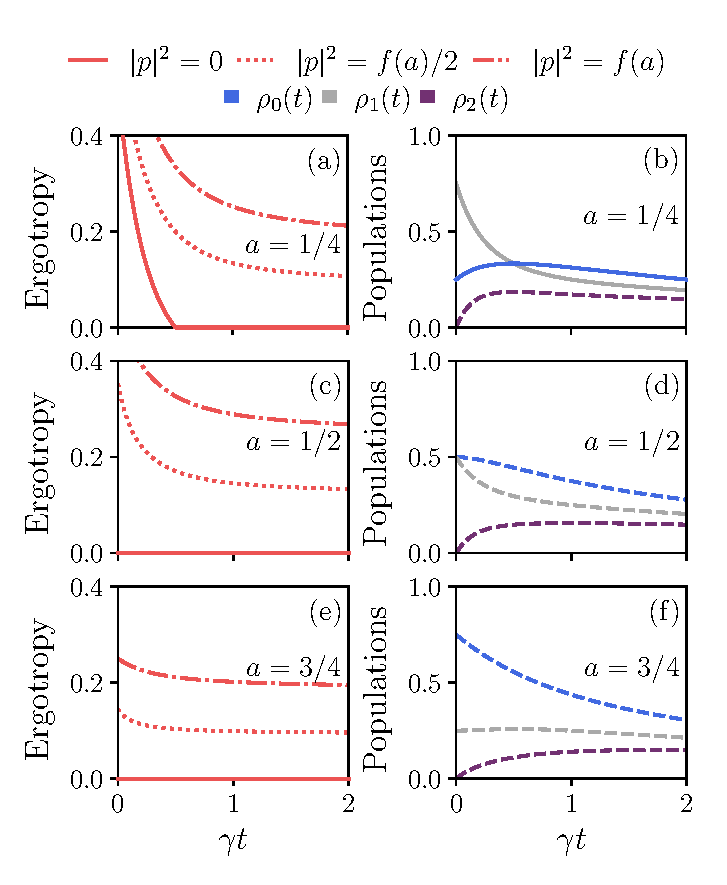
\includegraphics[width=\linewidth]{fig5.eps}
\caption{caption}
\label{fig5}
\end{figure}


\begin{figure}[H]
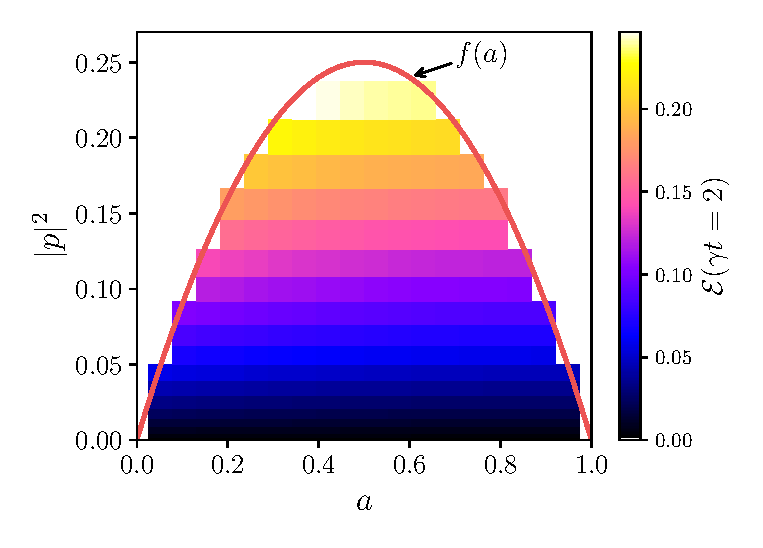
\includegraphics[width=\linewidth]{fig6.eps}
\caption{Colormap of ergotropy as a function of $a$ and $|p|^2$ for $\gamma t = 2$. The red line indicates the upper limit of $|p|^2$ imposed by the positivity condition of the density matrix.}
\label{fig6}
\end{figure}




\section{Conclusions}


 









% Appendix


\begin{acknowledgments}
We wish to acknowledge the financial support of CNPq (Conselho Nacional de Desenvolvimento Cient\'ifico e Tecnol\'ogico) and CAPES (Coordenação de Aperfeiçoamento de Pessoal de Nível Superior). 
\end{acknowledgments}

\appendix


% The \nocite command causes all entries in a bibliography to be printed out
% whether or not they are actually referenced in the text. This is appropriate
% for the sample file to show the different styles of references, but authors
% most likely will not want to use it.
%\nocite{*}

\bibliography{apssamp}% Produces the bibliography via BibTeX.

\end{document}
%
% ****** End of file apssamp.tex ******
